\chapter{Learning Theory Essentials}
\label{chap:learning_theory}

\begin{tldr}
This chapter covers learning theory concepts crucial for understanding why deep learning works: the bias-variance trade-off, double descent phenomenon, scaling laws, the lottery ticket hypothesis, grokking, and emergent abilities. These concepts are frequently discussed in staff-level interviews when evaluating model capacity and generalization.
\end{tldr}

\section{Bias-Variance Trade-off}
\label{sec:bias_variance}

\subsection{Classical View}

\begin{mathresult}{Bias-Variance Decomposition}
For squared error loss:
\begin{equation}
\E[(y - \hat{f}(x))^2] = \underbrace{\text{Bias}[\hat{f}(x)]^2}_{\text{underfitting}} + \underbrace{\Var[\hat{f}(x)]}_{\text{overfitting}} + \underbrace{\sigma^2}_{\text{irreducible}}
\end{equation}
\end{mathresult}

\textbf{Classical wisdom}:
\begin{itemize}
    \item Simple models: High bias, low variance (underfit)
    \item Complex models: Low bias, high variance (overfit)
    \item Optimal: Balance at intermediate complexity
\end{itemize}

\subsection{Why Deep Learning Breaks This}

Modern deep learning operates in a regime where:
\begin{itemize}
    \item Models have far more parameters than training examples
    \item Models can perfectly fit training data (zero training error)
    \item Yet they still generalize well!
\end{itemize}

This contradicts classical statistics and requires new understanding.

\section{Double Descent}
\label{sec:double_descent}

\subsection{The Phenomenon}

% \begin{figure}[H]
% \centering
% \begin{tikzpicture}
%     \begin{axis}[
%         xlabel={Model Complexity / Parameters},
%         ylabel={Test Error},
%         xmin=0, xmax=10,
%         ymin=0, ymax=3,
%         width=12cm,
%         height=6cm,
%         xtick={2.5, 5, 7.5},
%         xticklabels={Under-parameterized, Interpolation\\Threshold, Over-parameterized},
%         legend pos=north east
%     ]
    
%     % Classical U-curve
%     \addplot[domain=0:4.5, samples=50, thick, blue, dashed] {0.5 + 2*exp(-x) + 0.1*x^2};
    
%     % Double descent
%     \addplot[domain=0:4.8, samples=50, thick, red] {0.5 + 1.5*exp(-x) + 0.08*x^2};
%     \addplot[domain=4.8:5.2, samples=20, thick, red] {2.5 - 5*abs(x-5)};
%     \addplot[domain=5.2:10, samples=50, thick, red] {0.8 + 1.5*exp(-(x-5))};
    
%     \addlegendentry{Classical view}
%     \addlegendentry{Double descent}
    
%     % Interpolation threshold
%     % Interpolation threshold (moved outside axis)
%     \end{axis}
% \end{tikzpicture}
%     %\draw[dashed, gray] (5, 0) -- (5, 3);
%     %\node[above, font=\small] at (5, 2.8) {Interpolation};

    

% % \end{tikzpicture}
% \caption{Double descent: Test error peaks at interpolation threshold, then decreases again in over-parameterized regime.}
% \label{fig:double_descent}
% \end{figure}

\subsection{Three Regimes}

\begin{enumerate}
    \item \textbf{Under-parameterized} ($p < n$): Classical regime, bias-variance trade-off applies
    
    \item \textbf{Interpolation threshold} ($p \approx n$): Model barely fits training data, maximum variance, worst generalization
    
    \item \textbf{Over-parameterized} ($p \gg n$): Many solutions fit training data, optimization finds ``good'' ones
\end{enumerate}

\subsection{Why Over-parameterization Helps}

\begin{keyinsight}[Implicit Regularization]
In the over-parameterized regime:
\begin{enumerate}
    \item Many weight configurations achieve zero training loss
    \item Gradient descent with specific initialization finds solutions with small norm
    \item Small-norm solutions tend to be smoother and generalize better
\end{enumerate}
The optimization algorithm provides implicit regularization.
\end{keyinsight}

\section{Scaling Laws}
\label{sec:scaling_laws}

\subsection{Empirical Scaling Laws}

\begin{mathresult}{Kaplan et al. Scaling Laws}
Test loss follows power laws:
\begin{align}
L(N) &\propto N^{-\alpha_N} \quad \text{(parameters)} \\
L(D) &\propto D^{-\alpha_D} \quad \text{(data)} \\
L(C) &\propto C^{-\alpha_C} \quad \text{(compute)}
\end{align}
where $\alpha_N \approx 0.076$, $\alpha_D \approx 0.095$, $\alpha_C \approx 0.050$ for language models.
\end{mathresult}

\subsection{Chinchilla Scaling}

\begin{mathresult}{Chinchilla Optimal Scaling}
For a fixed compute budget $C$:
\begin{equation}
N_{opt} \propto C^{0.5}, \quad D_{opt} \propto C^{0.5}
\end{equation}
Optimal ratio: $D \approx 20N$ (tokens $\approx$ 20 × parameters)
\end{mathresult}

\textbf{Implication}: GPT-3 (175B params, 300B tokens) was undertrained. Chinchilla (70B params, 1.4T tokens) matches performance with less compute.

\subsection{Implications for Practice}

\begin{table}[H]
\centering
\caption{Scaling law implications}
\begin{tabularx}{\textwidth}{lX}
\toprule
\textbf{Finding} & \textbf{Practical Implication} \\
\midrule
Power law in parameters & 10× params → predictable improvement \\
Power law in data & More data always helps (diminishing returns) \\
Compute-optimal scaling & Balance model size and training data \\
Transfer across tasks & Scaling laws similar across domains \\
\bottomrule
\end{tabularx}
\end{table}

\section{The Lottery Ticket Hypothesis}
\label{sec:lottery_ticket}

\textbf{Lottery Ticket Hypothesis.} Dense, randomly-initialized networks contain sparse subnetworks (``winning tickets'') that, when trained in isolation from the same initialization, can match the full network's performance.

\subsection{Key Findings}

\begin{enumerate}
    \item \textbf{Existence}: Winning tickets exist (found via iterative pruning)
    \item \textbf{Initialization matters}: Must use original initialization, not random re-init
    \item \textbf{Sparsity}: Can prune 90-95\% of weights while maintaining accuracy
    \item \textbf{Transferability}: Tickets transfer across datasets (somewhat)
\end{enumerate}

\subsection{Implications}

\begin{itemize}
    \item Over-parameterization helps find good subnetworks
    \item Pruning after training can recover efficient models
    \item Motivates neural architecture search and efficient architectures
\end{itemize}

\section{Grokking}
\label{sec:grokking}

\textbf{Grokking.} The phenomenon where a model achieves perfect training accuracy long before achieving good generalization, with generalization suddenly improving much later in training.

\begin{figure}[H]
\centering
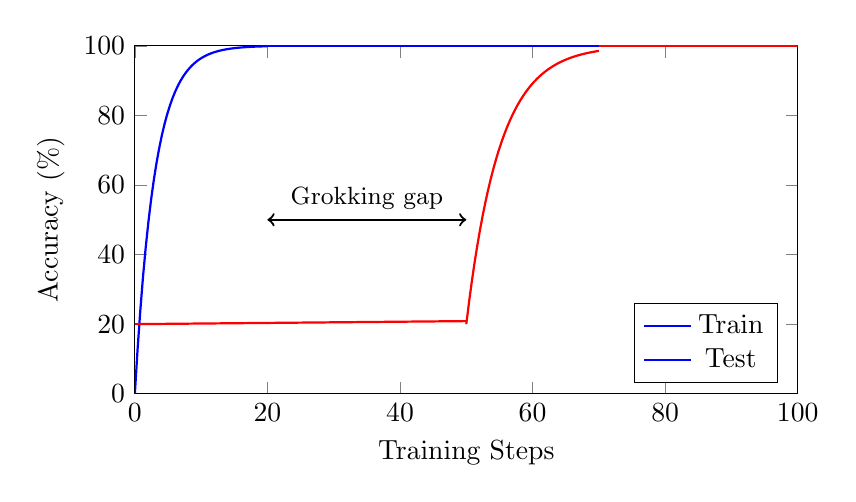
\begin{tikzpicture}
    \begin{axis}[
        xlabel={Training Steps},
        ylabel={Accuracy (\%)},
        xmin=0, xmax=100,
        ymin=0, ymax=100,
        legend pos=south east,
        width=10cm,
        height=6cm
    ]
    
    % Training accuracy
    \addplot[domain=0:20, samples=50, thick, blue] {100*(1 - exp(-x/3))};
    \addplot[domain=20:100, samples=50, thick, blue] {100};
    \addlegendentry{Train}
    
    % Test accuracy (grokking)
    \addplot[domain=0:50, samples=50, thick, red] {20 + 10*sin(x/10)};
    \addplot[domain=50:70, samples=50, thick, red] {20 + 80*(1 - exp(-(x-50)/5))};
    \addplot[domain=70:100, samples=50, thick, red] {100};
    \addlegendentry{Test}
    
    % Annotations
    \draw[<->, thick] (20, 50) -- (50, 50) node[midway, above, font=\small] {Grokking gap};
    
    \end{axis}
\end{tikzpicture}
\caption{Grokking: Training accuracy saturates early, test accuracy improves much later.}
\end{figure}

\subsection{When Grokking Occurs}

\begin{itemize}
    \item Small datasets with algorithmic structure (modular arithmetic)
    \item Heavy regularization (weight decay critical)
    \item Long training (much longer than needed for memorization)
\end{itemize}

\subsection{Proposed Explanations}

\begin{enumerate}
    \item \textbf{Representation learning}: Network first memorizes, then learns generalizable features
    \item \textbf{Circuit formation}: Generalizing circuits form slowly alongside memorizing circuits
    \item \textbf{Regularization dynamics}: Weight decay gradually removes memorization
\end{enumerate}

\section{Emergent Abilities}
\label{sec:emergent}

\textbf{Emergent Abilities.} Capabilities that appear suddenly at certain model scales, being absent in smaller models and present in larger ones, with sharp transitions rather than gradual improvement.

\subsection{Examples}

\begin{table}[H]
\centering
\caption{Examples of emergent abilities}
\begin{tabularx}{\textwidth}{lXr}
\toprule
\textbf{Ability} & \textbf{Description} & \textbf{Emerges at} \\
\midrule
In-context learning & Learn from examples in prompt & ~10B params \\
Chain-of-thought & Multi-step reasoning & ~100B params \\
Instruction following & Follow arbitrary instructions & ~10B params \\
\bottomrule
\end{tabularx}
\end{table}

\subsection{Debate on Emergence}

Recent work questions whether emergence is ``real'' or an artifact of:
\begin{itemize}
    \item Discrete evaluation metrics (accuracy shows sharp transitions)
    \item Continuous metrics (log-likelihood) show smooth improvement
    \item Task difficulty relative to model capability
\end{itemize}

\section{Implicit Regularization of SGD}
\label{sec:implicit_reg}

\subsection{Flat vs. Sharp Minima}

\begin{figure}[H]
\centering
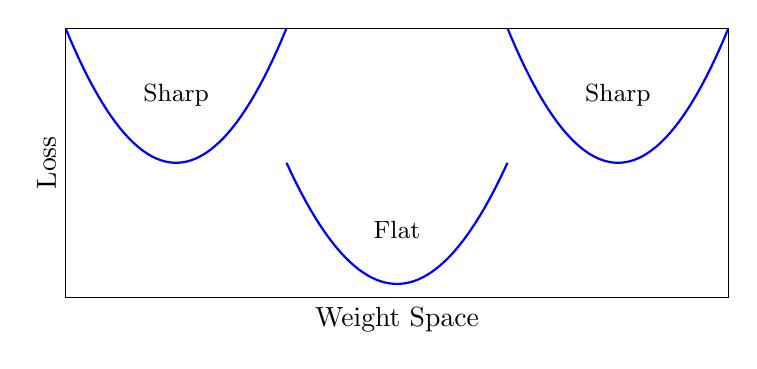
\begin{tikzpicture}
    \begin{axis}[
        xlabel={Weight Space},
        ylabel={Loss},
        xmin=-3, xmax=3,
        ymin=0, ymax=2,
        width=10cm,
        height=5cm,
        xtick=\empty,
        ytick=\empty
    ]
    
    % Sharp minimum
    \addplot[domain=-3:-1, samples=50, thick, blue] {1 + (x+2)^2};
    \addplot[domain=-1:1, samples=50, thick, blue] {0.1 + 0.9*(x)^2};
    \addplot[domain=1:3, samples=50, thick, blue] {1 + (x-2)^2};
    
    % Labels
    \node[font=\small] at (-2, 1.5) {Sharp};
    \node[font=\small] at (0, 0.5) {Flat};
    \node[font=\small] at (2, 1.5) {Sharp};
    
    % Arrows indicating generalization
    \draw[->, thick, green!70!black] (0, -0.3) -- (0, 0) node[below=0.3cm, font=\small] {Better generalization};
    
    \end{axis}
\end{tikzpicture}
\caption{Flat minima generalize better than sharp minima.}
\end{figure}

\subsection{Why SGD Finds Flat Minima}

\begin{enumerate}
    \item \textbf{Noise from mini-batches}: Gradient noise helps escape sharp minima
    \item \textbf{Learning rate}: Larger LR → more noise → flatter minima
    \item \textbf{Batch size}: Smaller batches → more noise → flatter minima
\end{enumerate}

\begin{keyinsight}
The ratio $\frac{\eta}{B}$ (learning rate / batch size) controls the ``temperature'' of SGD. Higher temperature explores more and finds flatter minima.
\end{keyinsight}

\subsection{Connection to Generalization}

Flat minima generalize better because:
\begin{itemize}
    \item Small perturbations (distribution shift) don't increase loss much
    \item Robust to noise in test data
    \item Often correspond to simpler functions
\end{itemize}

\begin{warningbox}
Classical statistical learning theory (VC dimension, Rademacher complexity) predicts over-parameterized models should overfit catastrophically. Deep learning violates these predictions routinely. In interviews, don't apply classical generalization bounds to deep networks---instead, discuss implicit regularization, double descent, and the role of optimization in finding good solutions.
\end{warningbox}

%==============================================================================
\section{Interview Questions}
\label{sec:learning_theory_interview}
%==============================================================================

\begin{interviewq}
\textbf{Q: Explain double descent. Why does test error decrease again in the over-parameterized regime?}

\textbf{What the interviewer is testing:} Whether you understand modern generalization theory beyond the classical bias-variance trade-off, and can explain why large models generalize well.

\textbf{A:} Double descent describes three regimes:
\begin{enumerate}
    \item \textbf{Under-parameterized} ($p < n$): Classical U-curve applies---more parameters initially reduce then increase test error.
    \item \textbf{Interpolation threshold} ($p \approx n$): The model barely fits training data, has maximum variance, worst generalization.
    \item \textbf{Over-parameterized} ($p \gg n$): Many solutions perfectly fit training data. Gradient descent with standard initialization finds solutions with small weight norm, which tend to be smoother and generalize better. This is \textit{implicit regularization}.
\end{enumerate}

The key insight: at the interpolation threshold, the model is forced into a unique (often bad) solution. With more parameters, there are many solutions, and SGD finds good ones.

\textbf{Common follow-ups:} ``Does double descent happen with epochs too?'' (Yes---epoch-wise double descent is also observed.) ``How does this relate to the lottery ticket hypothesis?'' (Over-parameterization helps find good subnetworks.)
\end{interviewq}

\begin{interviewq}
\textbf{Q: Your team has a fixed compute budget. How do you decide model size vs. training data?}

\textbf{What the interviewer is testing:} Knowledge of scaling laws and compute-optimal training (Chinchilla).

\textbf{A:} Chinchilla scaling tells us that for a fixed compute budget $C$, both optimal model size and optimal data scale as $C^{0.5}$. The practical rule is: \textbf{tokens $\approx$ 20$\times$ parameters}.

This means most early LLMs were undertrained. GPT-3 (175B params, 300B tokens) used a 1.7:1 ratio. Chinchilla (70B params, 1.4T tokens) matched its performance with 4$\times$ less inference cost because it used a 20:1 ratio.

\textbf{Practical implications:}
\begin{itemize}
    \item If you can't get more data, don't scale the model---you're wasting compute.
    \item For deployment, you want the smallest model that achieves your quality target, trained on maximum data.
    \item Recent work (LLaMA 3) shows you can train even beyond Chinchilla-optimal if inference cost matters more than training cost.
\end{itemize}

\textbf{Common follow-ups:} ``What if you have unlimited data but limited inference budget?'' (Train a smaller model longer---over-train relative to Chinchilla.) ``Do scaling laws transfer across domains?'' (Broadly yes, but exponents differ.)
\end{interviewq}

\begin{interviewq}
\textbf{Q: Are emergent abilities in LLMs real, or an artifact of evaluation?}

\textbf{What the interviewer is testing:} Critical thinking about ML claims, understanding of evaluation methodology.

\textbf{A:} This is genuinely debated. The original claim: certain capabilities (chain-of-thought, in-context learning) appear suddenly at specific model scales.

\textbf{The artifact argument} (Schaeffer et al., 2023):
\begin{itemize}
    \item Emergence appears with \textit{discrete} metrics (exact match accuracy) that show sharp transitions
    \item With \textit{continuous} metrics (log-likelihood, token-level accuracy), improvement is smooth and predictable
    \item The ``emergence'' is in the metric, not the model
\end{itemize}

\textbf{The reality argument}:
\begin{itemize}
    \item Even if continuous metrics improve smoothly, the qualitative capability (e.g., solving multi-step math) does appear suddenly in practice
    \item Composition of smoothly-improving sub-skills can produce emergent behavior
\end{itemize}

\textbf{Interview-safe answer}: Emergence is partly real and partly metric artifact. The important practical implication is that you can't reliably predict when a capability will appear, which makes evaluation at multiple scales essential.

\textbf{Common follow-ups:} ``How would you test if a capability is truly emergent?'' (Use continuous metrics, test at many scales, check if sub-skills improve smoothly.)
\end{interviewq}